

\chapter{Analysis of covariance (ANCOVA)}

Analysis of covariance (ANCOVA) is simply a regression with both continuous and categorical predictors. It has, however, a special application in situations in which we have "pre" and "post" scores.

\section{The meaning of the intercept}

Before we enter a categorical predictor, let us first example some properties of the intercept in models with paired $y$ and $x$ variables. Consider the hypothetical data in Table~\ref{tab:prepostdata}. This table has three columns, the first column is our post-test scores, the second column is our pretest scores, and the third column is the difference for reference. Since the "pre" and "post" tests are from the same units, we can compare the average change with a {\it paired} $t$-test
\begin{equation}
t=\frac{\bar{d}\sqrt{N}}{s_{d}}
\end{equation}
where $\bar{d}$ is the average difference (that is, the average of a new variable measuring the difference) and $s_{d}$ is the standard deviation of those differences. The result for the data in Table~\ref{tab:prepostdata} is $\bar{d}=9.4791$ and $s_{d} = 10.98465$ with 100 observations (which means the standard error of the difference is $\frac{s_{d}}{\sqrt{100}}=1.098465$). This leads to a $t$-value of 8.6294, which has a very small $p$-value.

How can we replicate this result with regression?

\subsection{As-is regression}

The idea is simple, suppose that there was no change, a scatter plot would simply be a diagonal line, as in Figure~\ref{fig:prepostsame}. If, however, on average respondents did change, then the line should rise or fall and this would be reflected in the intercept.

Thus, we may think we could fit the model
\begin{equation}
post_i = \beta_0 + \beta_1 pre_i + e_i
\end{equation}

and look at the intercept.

\begin{figure}
   \centering
   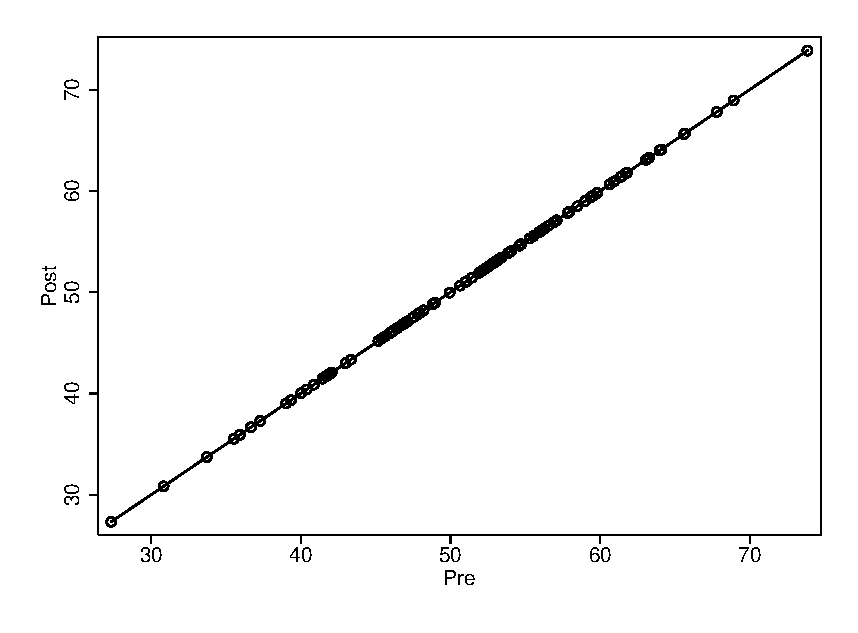
\includegraphics[angle=0,
           width=.75\textwidth]{prepostsame.eps}
   \caption{Scatter plot of data in which pre and post scores are the same with solid regression line}
  \label{fig:prepostsame}
\end{figure}

This thinking is adequate when the regression slope ($\beta_1$) for pre is approximately 1. However, the intercept is less telling about the change for the average pre score if the slope is greater or less than 1, as can be seen in Figure~\ref{fig:prepostalt}

\begin{figure}
   \centering
   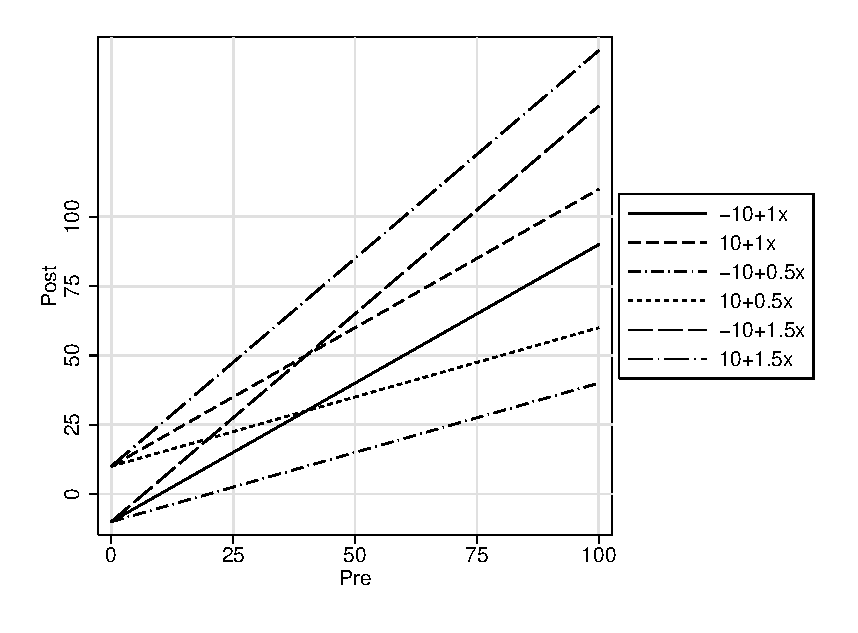
\includegraphics[angle=0,
           width=.75\textwidth]{prepostalt.eps}
   \caption{Different functions for pre-post regressions}
  \label{fig:prepostalt}
\end{figure}

A regression of post on pre, however, gives the difference for a low-scoring pre. This is reflected in Model 1 in Table~\ref{tab:prepostreg}, where the intercept is -12.498. This result is very different than the result of the paired $t$-test. The problem is that we are generally interested in the change for the {\it average} pretest, and the intercept reflects the change for a pre of 0.

\subsection{Regression on pre-centered variables}

If we center post and pre, on the {\it pre} mean,
\begin{equation}
post_i-\bar{pre} = \beta_0+\beta_1\left(pre_i-\bar{pre}\right)
\end{equation}
the intercept now reflects the average change for the average pre-test. This is reflected in Model 2 in Table~\ref{tab:prepostreg}. Note that in this case, $\beta_0$ is the result of the paired $t$-test. We can see the difference in Figure~\ref{fig:prepostreg}. When the data are not centered, the intercept is negative. However, by centering both the post and pre on the pre mean, we move the axis for $x$ and $y$ and now the intercept is positive. In general, this gives the {\it average} change for the {\it average} pre, which reflects the paired $t$-test difference.

\begin{figure}
   \centering
   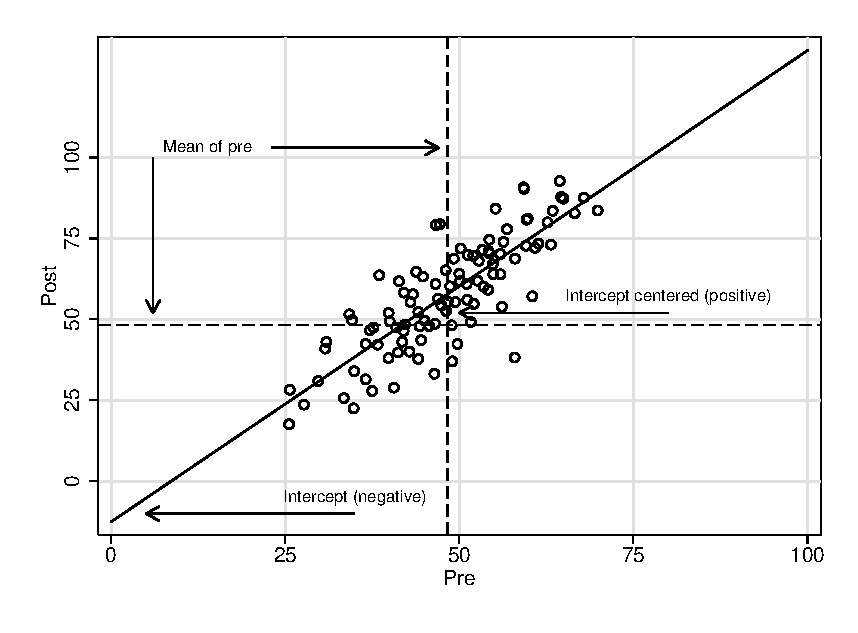
\includegraphics[angle=0,
           width=.75\textwidth]{prepostreg.eps}
   \caption{Scatter plot of data in Table~\ref{tab:prepostdata} with solid regression line and dashed reference lines}
  \label{fig:prepostreg}
\end{figure}

\subsection{Regression on the difference}

The first is to create a new variable that is the difference of post-pre and run an intercept only regression
\begin{equation}
post_i - pre_i = \beta_0 + e_i
\end{equation}
This is represented in Model 3 in Table~\ref{tab:prepostreg}, which reflects the result of the paired $t$-test.

\subsection{Why different standard errors for centered and difference models?}

Comparing Models 2 and 3 in Table~\ref{tab:prepostreg} you will notice that the standard errors for the intercept are different. To understand why, we need to remember where the standard error of intercepts comes from. The intercept is a predicted value (when $x$ is 0), and so like any other predicted value, the variance of the predicted value is equation~\eqref{eq:varfit}
\[
\mbox{var}\left(\hat{y}_0\right)=\left(\frac{\sigma^2}{N}+\frac{\left(x_0-\bar{x}\right)^2\sigma^2}{\sum_{i=1}^N\left(x_i-\bar{x}\right)^2}\right)\sigma^2
\]
and the standard error is
\begin{equation}
\mbox{SE}\left(\hat{y}_0\right)=\sigma\left(\frac{1}{N}+\frac{\left(x_0-\bar{x}\right)^2}{\sum_{i=1}^N\left(x_i-\bar{x}\right)^2}\right)^{1/2}
\end{equation}
which is governed by the residual variation $\sigma$ and the deviation from the mean. In the case of a centered model, the term $\frac{\left(x_0-\bar{x}\right)^2}{\sum_{i=1}^N\left(x_i-\bar{x}\right)^2}$ drops out, which leaves
\begin{equation}
\mbox{SE}\left(\hat{y}_0\right)^{centered}=\sigma\left(\frac{1}{N}\right)^{1/2}
\end{equation}
\begin{equation}
\mbox{SE}\left(\hat{y}_0\right)^{centered}=\frac{\sigma}{\sqrt{N}}
\end{equation}
which is the same as the variance of the mean, c.f. equation~\eqref{eq:meanvar}, and since $\sigma$ is smaller in Model 2 than in Model 3 (because we use the covariate), the standard error is smaller reflecting the use of more information.

\begin{table}[htbp]\centering
 \caption{Models to analyze differences between pre and post data in Table~\ref{tab:prepostdata}
\label{tab:prepostreg}}
\begin{tabular}{lccc}
\hline
Coefficients & Model 1 & Model 2 & Model 3 \\
\hline
Pre      &    1.455***&    1.455***&        \\
      &   (0.102)  &   (0.102)  &        \\
Intercept    &   -12.498* &    9.479***&    9.479***\\
      &   (5.035)  &   (1.007)  &   (1.098)  \\
\hline
\multicolumn{4}{l}{Model Statistics} \\
\hline
N      &   100.000  &   100.000  &   100.000  \\
F      &   202.700  &   202.700  &    0.000  \\
$R^2$     &    0.674  &    0.674  &    0.000  \\
$df$ Regression    &    1.000  &    1.000  &    0.000  \\
Sum of Squares Regression    &  20547.835  &  20547.835  &    0.000  \\
$df$ Error    &   98.000  &   98.000  &   99.000  \\
Sum of Squares Error     &  9934.307  &  9934.307  &  11945.602  \\
$\sigma$    &   10.068  &   10.068  &   10.985  \\
\hline
\multicolumn{4}{l}{Model 2 pre and post both centered on pretest mean} \\
\multicolumn{4}{l}{Model 3 predicts post-pre difference} \\
\multicolumn{4}{l}{$SE$s in parentheses, $*p<0.05, ***p<0.001$} \\
\hline
\end{tabular}
\end{table}

\subsection{Gains in power using regression technique}

A natural question is to ask under what circumstances using the regression technique is favorable. That is, when does it decrease standard errors by a measurable amount?

This can be answered with a quantity I call the PTIF for paired test inflation factor, which is
\begin{equation}
PTIF=\frac{1+v-2\rho\sqrt{v}}{\left(1-\rho^2\right)v}\times\frac{N-2}{N-1}
\end{equation}
where $\rho$ is the correlation between $y$ and $x$ $v$ is the ratio of the variance of $y$ to $x$. This quantity tells you how much larger the variance of the test is using the paired approach compaired to the the regression approach.

\section{ANCOVA: Bush election opinion example}

100 randomly sampled cases from the American National Election Study (2000 Pre- and Post-Election Survey) are presented in Table~\ref{tab:bushdata}. The cases are evenly divided among respondents who believed the outcome of the 2000 election was fair and those who believed it was not fair. Prior to the election and after things were settled, respondents were asked to give a temperature score (0-100) for several public figures, including G. W. Bush. The "before" and "after" columns are those scores that correspond the before and after the election, respectively.

Table~\ref{tab:bushmeans} presents the averages on the pre and post scores, and the average difference between post and pre (post-pre) by whether the respondents thought the election was fair.

\begin{table}[htbp]\centering
\caption{ Mean scores about G. W. Bush before and after 2000 election by whether election was fair
\label{tab:bushmeans}}
\begin{tabular}{lcccc}
\hline
Was election fair? & Score before election & Score after election & After - before \\
\hline
No &   55.84 &   51.50 &   -4.34 \\
Yes &   65.40 &   66.36 &    0.96 \\
\hline
  Total &   60.62 &   58.93 &   -1.69 \\
\hline
\end{tabular}
\end{table}

\subsection{Was there change, on average?}

We could of course perform a paired $t$-test

In this case the paired $t$-test is
\begin{equation}
t=\frac{\bar{d}\sqrt{N}}{s_{d}}
\end{equation}
\begin{equation}
t=\frac{-1.69\sqrt{100}}{18.44}
\end{equation}
\begin{equation}
t=-0.92
\end{equation}
Which has a standard error of the difference of 1.844 and results in a $p$ value of 0.36 with $N-1=99$ degrees of freedom.

\subsection{As-is regression}

As before we begin with a regression without centering. This is presented as Model 1 in Table~\ref{tab:bushreg}. If we take this model literally, we would believe that on average, the approval for Bush increased nearly 12 points from before the election to after. In fact, this is reflecting the change for persons who scored him at 0 before the election, and thus represents only regression towards the mean.

\subsection{Regression on pre-centered data}

Looking to Model 3 in Table~\ref{tab:bushreg}, our intercept again reflects the marginal difference in Table~\ref{tab:bushmeans} of -1.690, which in this case is not significant; but the standard error is smaller than the $t$-test. We can see the difference between the as-is regression and the pre-centered data in Figure~\ref{fig:bushscatter} and Figure~\ref{fig:bushscatterc}.

\begin{figure}
   \centering
   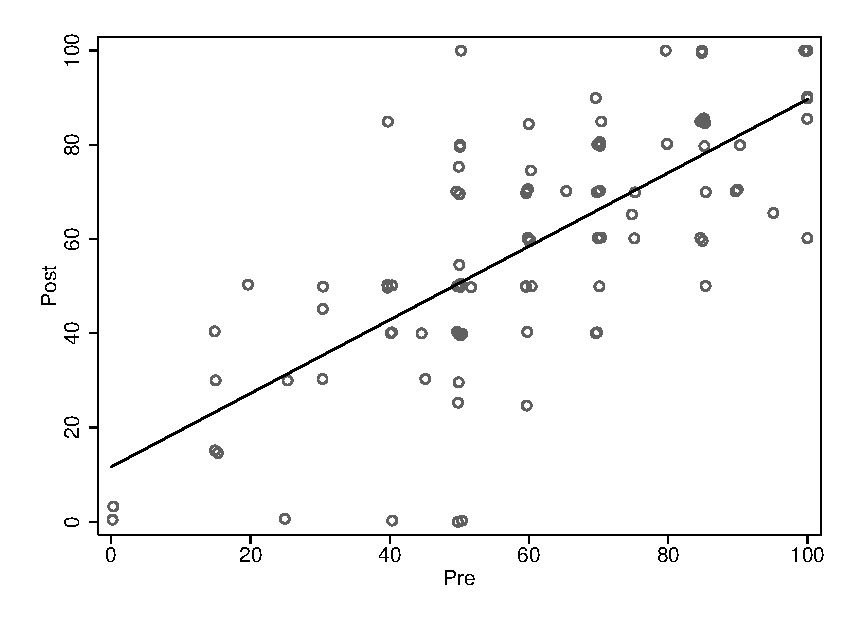
\includegraphics[angle=0,
           width=.75\textwidth]{bushscatter.eps}
   \caption{Scatter plot of data in Table~\ref{tab:bushdata} with regression line (note: small jitter added to points)}
  \label{fig:bushscatter}
\end{figure}


\begin{figure}
   \centering
   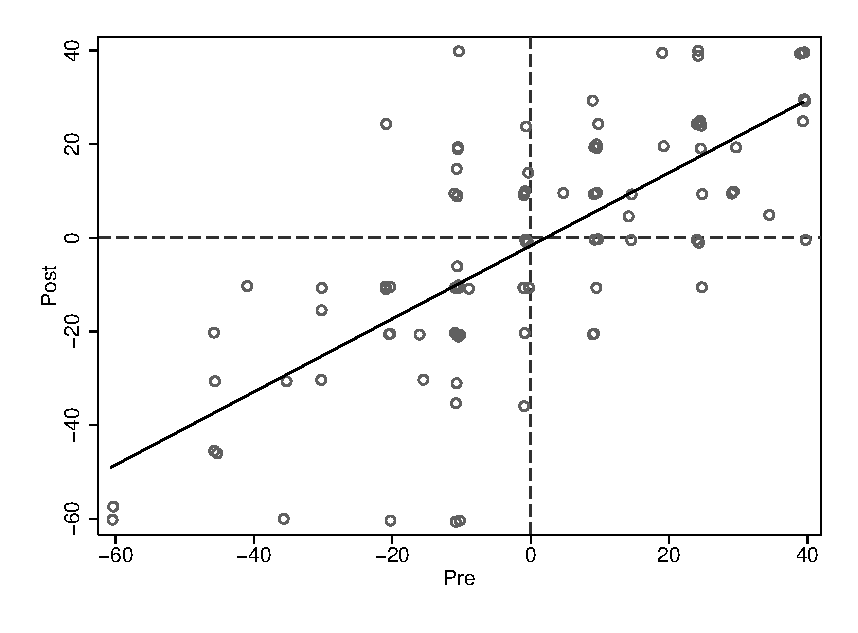
\includegraphics[angle=0,
           width=.75\textwidth]{bushscatterc.eps}
   \caption{Scatter plot of data in Table~\ref{tab:bushdata} (centered on pre mean) with regression line (note: small jitter added to points)}
  \label{fig:bushscatterc}
\end{figure}

\subsection{ANCOVA model: adding a categorical covariate}

Now things get interesting. We can now ask ourselves if believing the election was fair influenced the impact on respondents from before to after the election. Adding in the simple covariate, a dummy variable indicating whether the respondent felt the election was fair, leads to Models 2 and 4 in Table~\ref{tab:bushreg}. In both models, the effect of believing the election was fair yields the same result, model fit, etc. However, the intercept in Model 2 would lead us to believe that there was no change for those who felt the election was not fair. However, this again reflects individuals who scored Bush as 0 on the pre score. Using the centering technique, we instead find that for a person who thought the election was unfair, but had the global average on the pretest, their opinion of Bush decreased 5.556 points. Those who believed the election was fair increased -5.556+7.733=2.177 points.

In order to replicate the results in Table~\ref{tab:bushmeans}, we would need to center pre and post on the pre means specific to the categorical variable. We do this in Model 5 in Table~\ref{tab:bushreg}. In that case, the intercept is -4.34, and the effect of fair is 5.3, for a difference specific to those who thought the election was fair of -4.34+5.3 = 0.96, which is reflected in the means table. Unfortunately, by removing the mean differences due to the fairness indicator, we are no longer comparing the same pretest and our results are no longer significant.

\subsubsection{Lord's paradox}

Which is the correct method? If we centered on the within-group means, we find no effect. If we center on a global mean, we find an effect. This is the crux behind the famous Lord's paradox, named after Frederic M. Lord who called attention to it in 1967. There is no apparent answer, except to be explicit on the research question and use the correct means when centering.

\begin{table}[htbp]\centering
 \caption{Models to analyze differences between pre and post election scores for G. W. Bush
\label{tab:bushreg}}
\begin{tabular}{lccccc}
\hline
Coefficients & Model 1 & Model 2 & Model 3 & Model 4 & Model 5 \\
\hline
Pre  &    0.780***&    0.746***&    0.780***&    0.746*** & 0.746*** \\
      &   (0.077)  &   (0.077)  &   (0.077)  &   (0.077) & (0.077) \\
Fair    &        &    7.733* &        &    7.733* & 5.300 \\
      &        &   (3.575)  &        &   (3.575) & (3.497)  \\
Intercept    &   11.640* &    9.869  &   -1.690  &   -5.556* & -4.340 \\
      &   (4.997)  &   (4.974)  &   (1.781)  &   (2.500) & (2.472) \\
\hline
\multicolumn{6}{l}{Model Statistics} \\
\hline
N      &   100.000  &   100.000  &   100.000  &   100.000 & 100.00 \\
F      &   102.575  &   55.553  &   102.575  &   55.553 & 47.674  \\
$R^2$     &    0.511  &    0.534  &    0.511  &    0.534 & 0.496 \\
$df$ Regression    &    1.000  &    2.000  &    1.000  &    2.000 & 2.000 \\
Sum of Squares Reg.    &  32542.960  &  33973.928  &  32542.960  &  33973.927 & 29155.688  \\
$df$ Error    &   98.000  &   97.000  &   98.000  &   97.000 & 97.000  \\
Sum of Squares Error     &  31091.550  &  29660.582  &  31091.549  &  29660.582 & 29660.582  \\
\hline
\multicolumn{5}{l}{Model 3 pre and post centered on pretest mean } \\
\multicolumn{5}{l}{Model 4 pre and post centered on pretest mean } \\
\multicolumn{5}{l}{Model 5 pre and post centered on pretest mean within group} \\
\multicolumn{5}{l}{$SE$s in parentheses, $*p<0.05, ***p<0.001$} \\
\hline
\end{tabular}
\end{table}